\documentclass[12pt,xcolor=svgnames]{beamer}

\usepackage{natbib}
\usepackage{xspace}
\usepackage{graphics}
\usepackage{graphicx}
\usepackage{url}
\usepackage{datetime} % an add-on.  get from CTAN, with fmtcount
\usepackage{multimedia}
\usepackage{multirow}
\usepackage{listings}
\usepackage{setspace}
\usepackage{amsmath} % [For split environment: When used inside equation, allows multiple lines with a single equation number, align with &'s.]
%\usepackage{listings} % for source code listings
%\usepackage{subfigure}
%\usepackage{wrapfig} % allows wrapping text around figures
%\usepackage{amssymb}
%\usepackage{hyperref}

% MARSHALL'S CONFIG STUFF
\newcommand{\ie}{i.e.\@\xspace}
\newcommand{\eg}{e.g.\@\xspace}
\newcommand{\cf}{cf.\@\xspace}
\newcommand{\etc}{etc.\@\xspace}
\newcommand{\viz}{viz.\@\xspace}
\newcommand{\vs}{vs.\@\xspace}
\newcommand{\fn}[1]{\footnote{#1}}
\newcommand{\cmnt}[1]{}
%\renewcommand{\cmnt}[1]{{\color{red}\footnotesize [#1]}}
\newcommand{\bgcmnt}[1]{} % ones I don't normally want to see
\newcommand{\pr}{\mathsf{P}} % probability
\newcommand{\relf}{\mathsf{R}} % probability
%\newcommand{\expct}{\mbox{\boldmath $\mathsf E\,$}}
\newcommand{\expct}{\mathsf E\,}
%\newcommand{\var}{\sigma^2}
%\newcommand{\var}{\mathop{\mathrm{var}}\nolimits}
\newcommand{\notbar}[1]{\overline{#1}}
\newcommand{\pri}{\pr_{\cal I}}      % input probability
%\newcommand{\pro}{\pr_{\cal O}}      % output probability
\newcommand{\proff}[2]{\mathsf{P}(O_{#1}={#2})} % pr num offspring #1 = #2
%\newcommand{\fitness}[1]{\mbox{Fitness of $#1$}}
%\newcommand{\cfitness}[2]{\mbox{Fitness of $#1$ given the occurrence of $#2$}}
\newcommand{\fitfn}{\mathsf F}
%\newcommand{\fitfn}{\,\mathsf w}
\newcommand{\Do}{\mathsf{do}}
\newcommand{\arw}{$\leftrightarrow$}

% % space between items:
% \newlength{\wideitemsep}
% \setlength{\wideitemsep}{\itemsep}\addtolength{\wideitemsep}{3pt}
% % reconfigure itemize lists:
% \let\olditem\item
% \renewcommand{\item}{%
% \setlength{\itemsep}{\wideitemsep}%
% \olditem}
% OR:
\let\olditem\item
\renewcommand{\item}{%
\olditem\vspace{0.5pt}}

\newcommand{\Note}[1]{\note{#1\ \\ \ \\}} % uses beamer \note command see ch19

\newcommand{\sectionframe}[1]{%
\section{#1}
\begin{frame}
\begin{beamercolorbox}{title}
\centering\usebeamerfont{title}\LARGE #1
\end{beamercolorbox}
\end{frame}}

%\usetheme{OnHand} % doesn't have latest updates?
%\usetheme{OnHans}
%\usetheme{OnFoot}
\usetheme{OnTheFly}
%% for e.g. EB Garamond:
% \addfontfeatures{Numbers=Lining}
% \newcommand{\one}{\mbox{\lnum{1}}} % kludge for lining 1 in math mode
%% for Garamond No8:
\newcommand{\one}{1}

%\setbeamercovered{transparent} % show faint versions of hidden items
%\setbeamercovered{transparent=0} % control degree of fadedness (default 15)
%\setbeamercovered{dynamic} % later items might be harder to see until close
\setbeamercovered{invisible}


\newcommand{\theTitle}{Humanistic Computer Simulations}

%\newcommand{\flatTitle}{\theTitle}

\title[\theTitle]{\theTitle}

\author{Marshall Abrams}

\institute[UAB]{
Department of Philosophy\\
University of Alabama at Birmingham\\
\ \\
THATcamp Alabama 2014
}

\date{September 6, 2014}

\setbeameroption{hide notes}
%\setbeameroption{show notes}
%\setbeameroption{show only notes}
%\setbeameroption{show notes on second screen=<location>}
%
% NOTE if notes are shown with my OnFoot or related beamerthemes,
% then the line that puts the section into the header,
%      {\usebeamerfont{section in head/foot}\usebeamercolor[fg]{section in head/foot}\hfill\scriptsize\insertsectionhead\hspace{8pt}\strut\par}%
% will cause warning messages from Xelatex, I think because the
% section name is too close to the edge in the little thumbnail
% of the page.  Now you (I) know.

\begin{document}

\begin{frame}%
  \titlepage%
  \Note{PREP: power cable\\
  NetLogo (two copies, two sims?)\\
  Two movies\\
  text file text/crimepropns.nt1\\
  text file text/crime3withnotes.lisp\\
  or sanday
  }
\end{frame}

\section{Introduction}

\begin{frame}\frametitle{Some humanities simulations}
\vspace{-1ex}
\footnotesize\begin{itemize}
\item structural patterns of narratives in 19th C. novels
\item how literary genres evolve over time
\item why the Anasazi people disappeared from American Southwest mid-14th C.
\item how scientific theories change over time
\item origin of vague concepts, development of linguistic conventions
\item the development of morality 
\item how culture spreads given innovation, teaching, biases
\item how consensus and disagreement arise.
\item historical publishing and letter transmission networks
\item Ancient Roman faction conflicts
\item 19th C. Battle of Trafalgar
\item Medieval military logistics
\end{itemize}
\end{frame}


%\begin{frame}\frametitle{Where does this come from?}
\begin{frame}\frametitle{Origins}
\begin{itemize}
\item NEH's ``humanities"\Note{2011 NEH summer institute on
    Computer Simulations in the Humanities}
\item I am an ``analytic" philosopher of science\Note{humanist or
    scientist?}, with interests in
    \begin{itemize}
    \item mathematical/computer models in evolutionary biology
    \item in cognitive science
    \item in anthropology
    \end{itemize}
    %
\item How can scientific social sciences become more
    ``humanistic"---without becoming less
    scientific?\Note{Pinker\ldots}
\end{itemize}
\end{frame}

\begin{frame}\frametitle{Interpretation and modeling}
Humanities: insights from interpretation, analogy,
    structural relationships, \eg between  specific
    instances.\Note{humanities: loose structural patterns}
%
\begin{quote}\small
    His talent was as natural as the pattern that was made by the
    dust on a butterfly's wings.  At one time he understood it no
    more than the butterfly did and he did not know when it was
    brushed or marred.  Later he became conscious of his damaged
    wings and of their construction and he learned to think and
    could not fly anymore because the love of flight was gone
    and he could only remember when it had been effortless.\\
    \ \\
\footnotesize (\citealt{Hemingway:MoveableFeast}, quoted in \citealt[223]{HolyoakThagard:MentalLeaps})
\end{quote}
\Note{On F. Scott Fitzgerald}
\end{frame}

\begin{frame}\frametitle{Interpretation and modeling}
\begin{itemize}
\item Math: insights from precise, abstract structural relationships
\end{itemize}
\Note{Math is about precise structural parallels.  Precise
analogies.}
\end{frame}

\begin{frame}\frametitle{Interpretation and modeling}
\begin{itemize}
\item Mathematical modeling in science: precise formulation, loose relationships
\Note{Models are analogies.  \cf Hesse {\em Models and Analogies in
Science\/} \citeyearpar{Hesse:ModelsAnalogies}}
\end{itemize}
\Note{In this talk I'm using analogies between 
scientific and philosophical domains. 
Humanities methods applied to science and philosophy.}
\end{frame}

\begin{frame}\frametitle{Evolutionary biologists \ldots}
Use mathematical models\\
\ \\
to study abstract patterns of change over time\\
\ \\
in populations of organisms,\\
\ \\
including, sometimes, spread of genetic patterns.
\end{frame}

\begin{frame}\frametitle{Social scientists \ldots}
Use mathematical models\\
\ \\
to study abstract patterns of change over time\\
\ \\
in populations of people,\\
\ \\
including, sometimes, spread of cultural patterns.
\end{frame}


\begin{frame}\frametitle{The Modeling Strategy}
Try to approximate structural patterns with precise models,\\
\ \\
\ \\
\ \\
recognizing that other dimensions of the subject are left out.\\
\ \\
\ \\
\ \\
\Note{cf. a lot of digital humanities}
\Note{This doesn't ``reduce" or deny the importance of
traditional methods in the humanities, etc., which capture
dimensions, richness that modeling and other science-inspired
methods have trouble capturing (but we can try ...)}
\end{frame}


\begin{frame}\frametitle{Modeling meaning?} 
Historian Stuart Clark on Medieval reports of demonic possession:
\begin{quote}
    \small For it is a defining feature of cultural
    forms that the actions they warrant only exist at all as
    actions of a certain sort because of the properties
    arbitrarily conferred on them by systems of representation. 
    We can, therefore, extrapolate what was physical in
    possession behaviour and make it yield explanations in a
    different context only if we divorce it from precisely those
    semantic circumstances that enable victims and observers at
    the time to say (and argue about) just what it was.
    \citep[p.\ 410]{Clark:ThinkingWithDemons}
\end{quote}\vspace{-1ex}
\ie Treating possessions as \eg physiological phenomena 
misses what they really are, in another sense.  Seeing that
requires understanding religious texts and traditions.
\Note{I see the processes in each agent as {\em models of\/}
cognitive processes.  But it's a {\em model\/}.  Maybe you can
{\em just\/} view it as a model of meanings, as long as you're
willing to say that there is an analogous pattern to relations between
meanings and communciation.}
\end{frame}

\section{Agent-based culture models}

\begin{frame}\frametitle{What is agent-based modeling?}
\begin{itemize}
\item Rather than a computer program with a master plan
\item Let outcomes emerge from the interaction from many\\
relatively simple ``agents".\Note{Sometime not always
agents are abstract reps of humans---idealizations, abstractions,
capturing abstract patterns of human interactions}
\item These outcomes reflect structural assumptions embedded
within the agents.
\item How-possibly insights: What could explain this?  If they're
abstract patterns, let's simulate them.
\item Predictions when well calibrated to initial conditions.
\end{itemize}
\ \\
\ \\
\ \\
\begin{center}\footnotesize (CultranDejanet.nlogo: 
200, 10; 125, 35)\end{center}
\Note{
Degrees of confidence are not transmitted. Instead, the degree of
confidence (activation) determines the probability that a belief
will be communicated. (After all, when people offer assertions to
each other, they don’t generally indicate their degree of confidence,
even if there are ways to do that by choice of words and tone of
voice.)

On each tick, for each link attached to a person, the person randomly
decides to “utter” the proposition to its (undirected) network
neighbors, with probability equal to the absolute value of the
degree of confidence plus transmission-bias-prob. The value that’s
conveyed to the receiver of the utterance is trust-mean times the
sign of the original degree of confidence, or a normally distributed
value with mean trust-mean and standard deviation trust-stdev, if
trust-stdev is not zero. The effect of this input to the receiver’s
degree of confidence depends on how far the latter is from -1 or
1.}
\Note{EXAMPLE HERE\\
CultranDejanet: v1: 200 nodes, degree=10; v2: 125 nodes, degree=35\\
Lansing-Kremer}
\end{frame}


\begin{frame}\frametitle{Kinds of agent-based models}
\begin{itemize}
\item Simple agent: Agents' internal rules/processes are not complex.
\item Complex agent: Agents' internal rules/processes are complex.
\item Moderate-complexity agent: In between.
\end{itemize}
\ \\
\ \\
Tradeoffs between understanding and realism.
\Note{Moderate-complexity models are tricky, but have the potential to
grab onto additional humanistic richness.}
\end{frame}


\begin{frame}\frametitle{Cultural variant-variant interactions}
\begin{itemize}
\item Culture viewed as integrated whole
\item Yet cultures differ
\item And social entities are made of people---who differ.
\item How does such a complex, rich, integrated messy whole come about?
\end{itemize}
\Note{EXAMPLE HERE:
CultranDejanet: v1: 200 nodes, degree=10; v2: 125 nodes,
degree=35}
\end{frame}

\begin{frame}\frametitle{Cultural variant-variant interactions}
\begin{itemize}
\item Interactions between cultural variants, and environmental
factors, affect transmission\\
\ \\
        Logical, analogical, association, emotional, ``symbolic"
        relations\\
\ \\
e.g. Geertz argued that relationships in Balinese cockfighting
represent social and emotional relations between people, families, etc.
\end{itemize}
\Note{Cognitive dissonance, epistemological coherence, ``Freedom", cockfight/social relats, subaks, 
\citep{Gonzalez:ZapotecScience}
Gonzalez peasant food, Clark demons, Hofstadter/Sander
(Lakoff).\\
I think that many subtle interactions in culture can be viewed as
involving analogy, abstract pattern matching.  So that's what I'm
pursuing.}
\end{frame}


\begin{frame}\frametitle{Analogical interaction}
Thibodeau and Boroditsky
\citeyearpar{ThibodeauBoroditsky:MetaphorsThinkWith,
ThibodeauBoroditsky:MetaphorsInfluenceReasoning}
showed Americans two versions of a paragraph about crime in a city,
varying one word:
\begin{quote}
{\small ``Crime is a \{beast/virus\} ravaging the city of Addison."}
\end{quote}
Then asked what should be done.
\begin{itemize}
\item Participants who saw ``beast" recommended {\em capture\/} and
    punishment solutions relatively more often than 
\item participants who saw ``virus", who were relatively more
likely to suggest solutions involving financial, educational
support, {\em isolating\/} individuals at risk from existing criminals.
\end{itemize}
%\tiny
%\begin{quote}
%Crime is a \{beast/virus\} ravaging the city of Addison. Five
%years ago Addison was in good shape, with no obvious
%vulnerabilities. Unfortunately, in the past five years the city’s
%defense systems have weakened, and the city has succumbed
%to crime. Today, there are more than 55,000 criminal
%incidents a year---up by more than 10,000 per year. There is
%a worry that if the city does not regain its strength soon, even
%more serious problems may start to develop.\\
%\citep{ThibodeauBoroditsky:MetaphorsThinkWith}
%\end{quote}
%
\end{frame}

\begin{frame}\frametitle{Analogical interaction}
%A framing effect due to priming by culturally-specific cross-domain
%analogical relationships:
\begin{itemize}
\item Beliefs about viruses and aggressive animals
\item affect beliefs about crime
\item due to metaphorical/analogical relationships.
\end{itemize}
\vspace{3ex}
Plausibly, such analogical effects are commonplace \\
%and can affect transmission
{\scriptsize (\cf \citealt{HofstadterSander:SurfacesEssences,
Lakoff:MoralPolitics, GentnerEtAl:MetaphorLikeAnalogy})}.
\end{frame}


%\begin{frame}\frametitle{Analogy can be adaptive}
%How to destroy tumor deep inside body using beams of radiation
%without destroying good tissue?\\
%\ \\
%\uncover<2,3,4>{Roads to dictator's fortress protected by land mines
%insensitive to low-intensity vibrations.
%How can revolutionary army attack?}\\
%\ \\
%\uncover<3,4>{Split army into small groups, each taking a different 
%road to the fortress.}
%\ \\
%\ \\
%\uncover<4>{Do the ``same" thing with the tumor problem.\\
%{\scriptsize \citep{GickHolyoak:AnalogicalProbSolving,
%HolyoakThagard:MentalLeaps, Duncker:OnProbSolving}}}
%\end{frame}

%\begin{frame}\frametitle{Analogy as adaptive}
%Analogy:
%\begin{itemize}
%\item Generates complex hypotheses for reasoning, trial-and-error
%investigation.\\
%\item Facilitates adaptation in dispersal and environmental change.
%\item Aids communication, recollection.\\
%\item Plausibly underlies many symbolic cultural relationships\\
%{\tiny (cf. Geertz's account of Balinese cockfight).}
%\end{itemize}
%\end{frame}

\begin{frame}\frametitle{Analogy as adaptive}
Analogy:
\begin{itemize}
\item Is a source of creativity and tool for problem-solving,
\eg in new contexts.
\item Aids communication, recollection.\\
\item Plausibly underlies many symbolic cultural relationships\\
{\tiny (cf. Geertz's account of Balinese cockfight).}
\end{itemize}
\end{frame}

\begin{frame}\frametitle{What is analogy}
\begin{center}\vspace{-5ex}
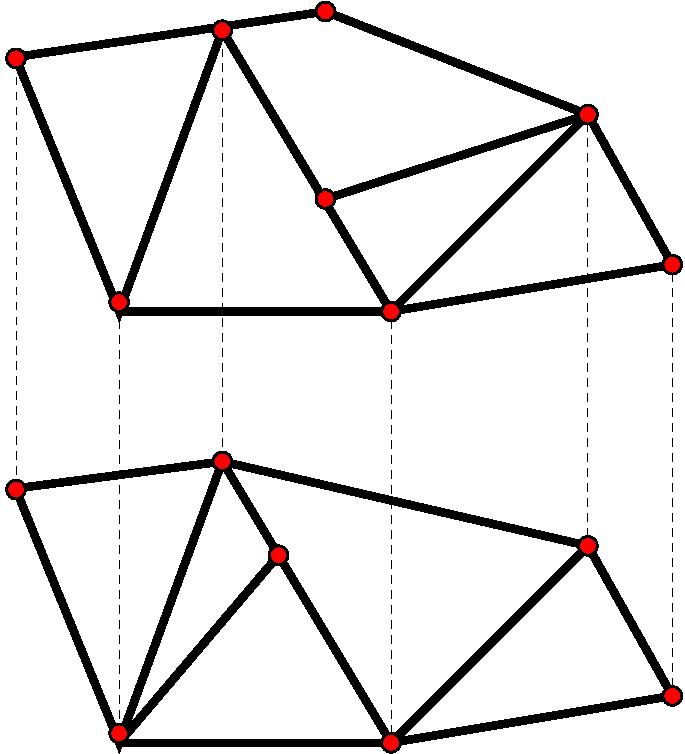
\includegraphics[scale=.2]{../figures/analogyVisualAnalogy.pdf}\\
\end{center}\vspace{-3ex}
\begin{itemize}
\item A ``good" analogy maps elements (properties, objects,
    propositions) of one domain to elements of another,
preserving structural relations as well as possible.
\item An isomorphism-like relation (roughly: structure-preserving)
\item Higher-order pattern matching
\end{itemize}
\citep{Gentner:StruMappingThFramework,
Holyoak:FrameworkLiteraryInterp,
Hofstadter:FluidConcepts}
\Note{
\begin{itemize}
\item as all teachers know.
\item \eg Geertz: Patterns of interaction and emotions in
    Balinese cockfights as ``analogy" for those in coalitions and
    rivalries.  Sanday.
\item GOAL OF SIMULATIONS: Show analogy as a bias on
    probabilistic processes of cultural change.
\item \cf \citep*{PennHolyoakPovinelli:DarwinsMistake} 
\end{itemize}
}
\end{frame}

\begin{frame}\frametitle{POPCO example}
\begin{itemize}
\item 3 populations
\item 40 persons per population speaking about crime.
\item Who talks to whom is random.
\item What each says is affected by beliefs.
\item The world intermittently tells everyone that each crime proposition is true.
\item Populations:
\begin{itemize}
\item {\em beast\/} bias: everyone has beast analog (not virus)
\item {\em virus\/} bias: everyone has virus analog (not beast)
\item {\em both\/} bias: everyone has both analogs
\end{itemize}
\item Processes within each person are deterministic.
\end{itemize}
\end{frame}

\begin{frame}\frametitle{Degrees of beliefs, 6 popco persons}
\vspace{-3ex}
\makebox[\textwidth][c]{%
\begin{tabular}{ccc}
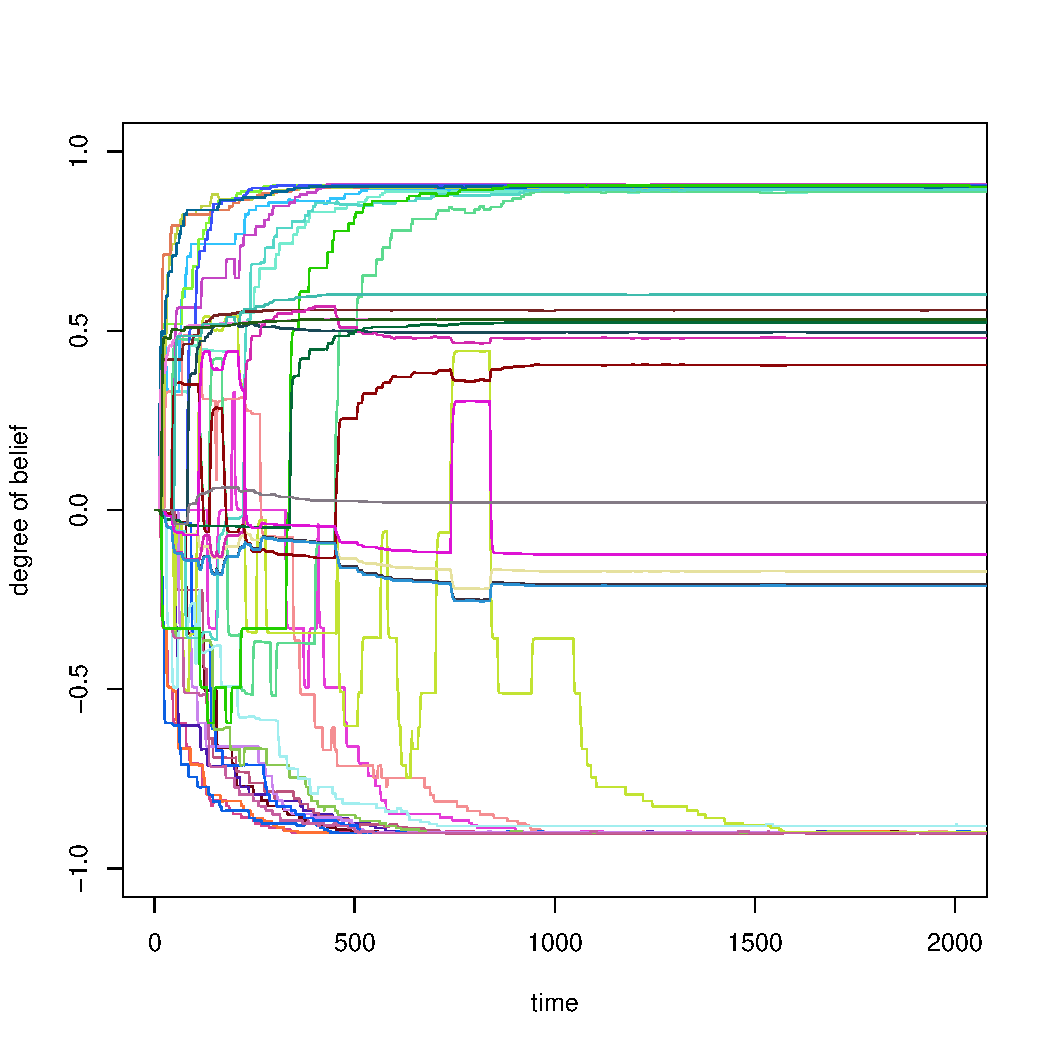
\includegraphics[scale=.20]{../figures/mra3b2p2000ticksRUN387661242P01} & 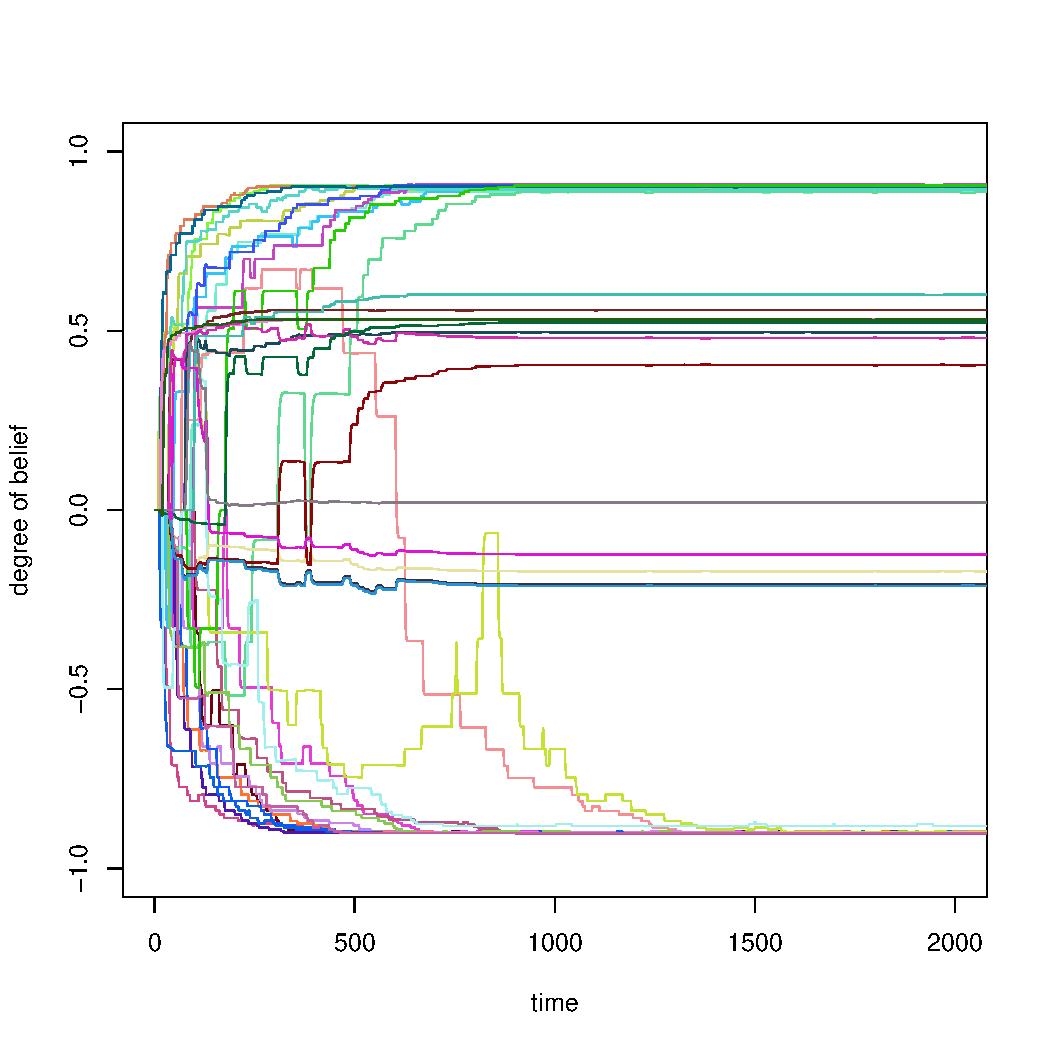
\includegraphics[scale=.20]{../figures/mra3b2p2000ticksRUN387661242P02} & 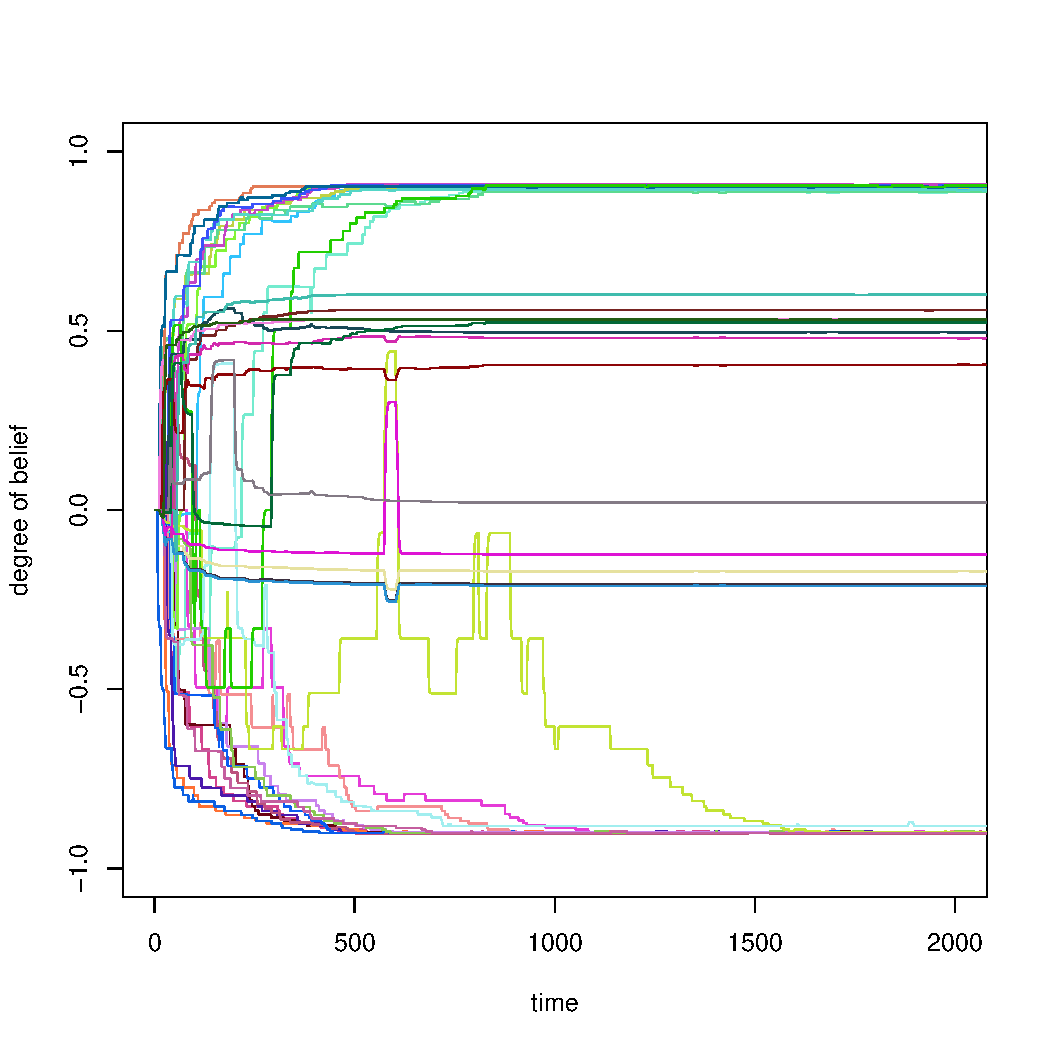
\includegraphics[scale=.20]{../figures/../figures/mra3b2p2000ticksRUN387661242P03} \\
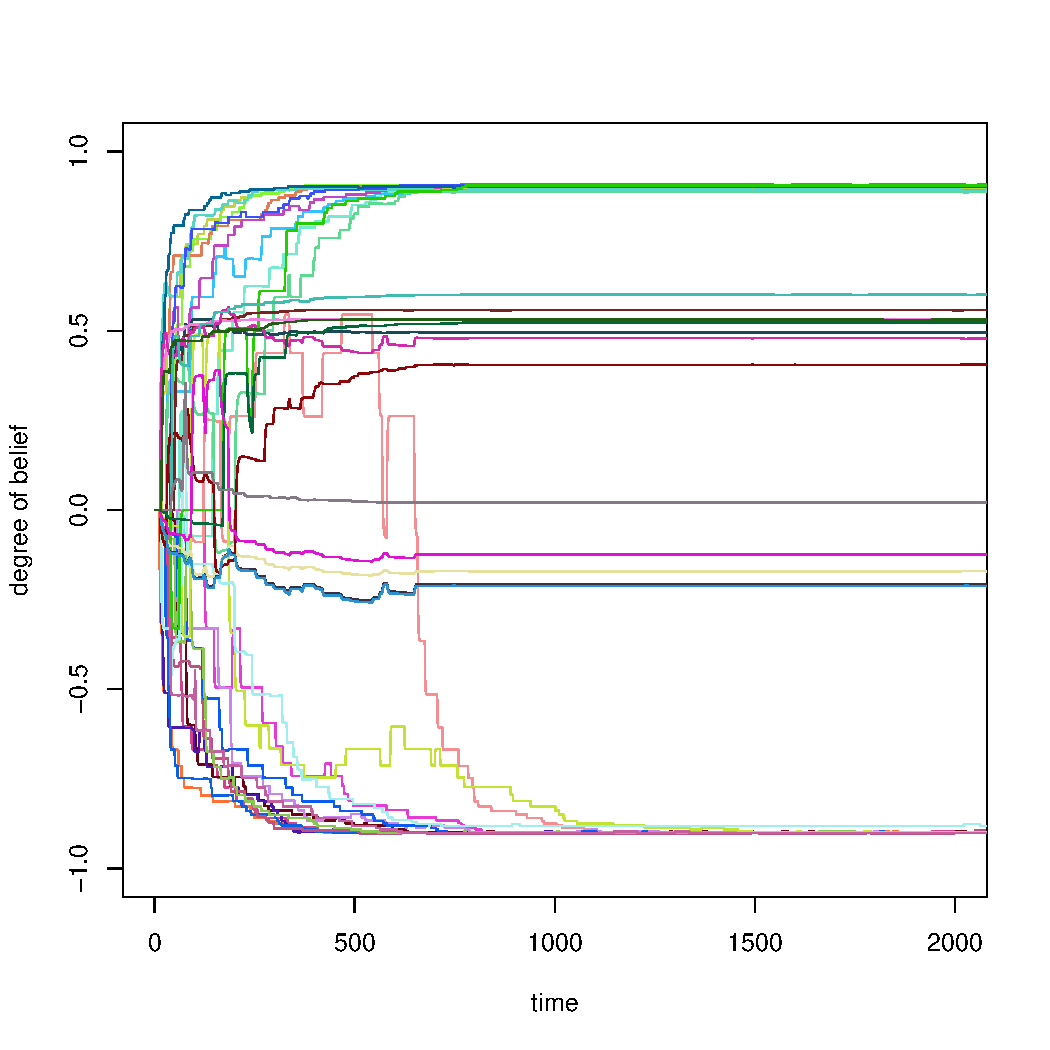
\includegraphics[scale=.20]{../figures/mra3b2p2000ticksRUN387661242P04} & 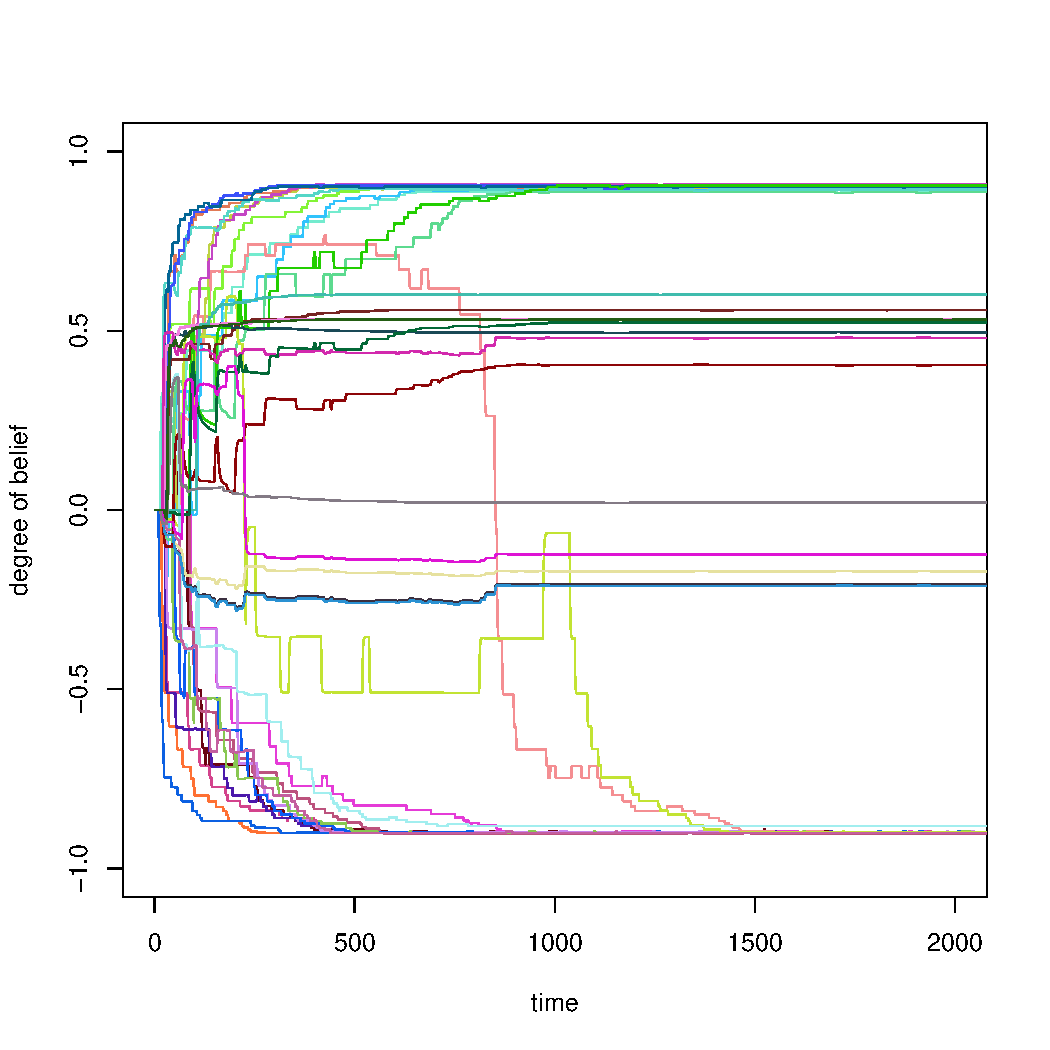
\includegraphics[scale=.20]{../figures/mra3b2p2000ticksRUN387661242P16} & 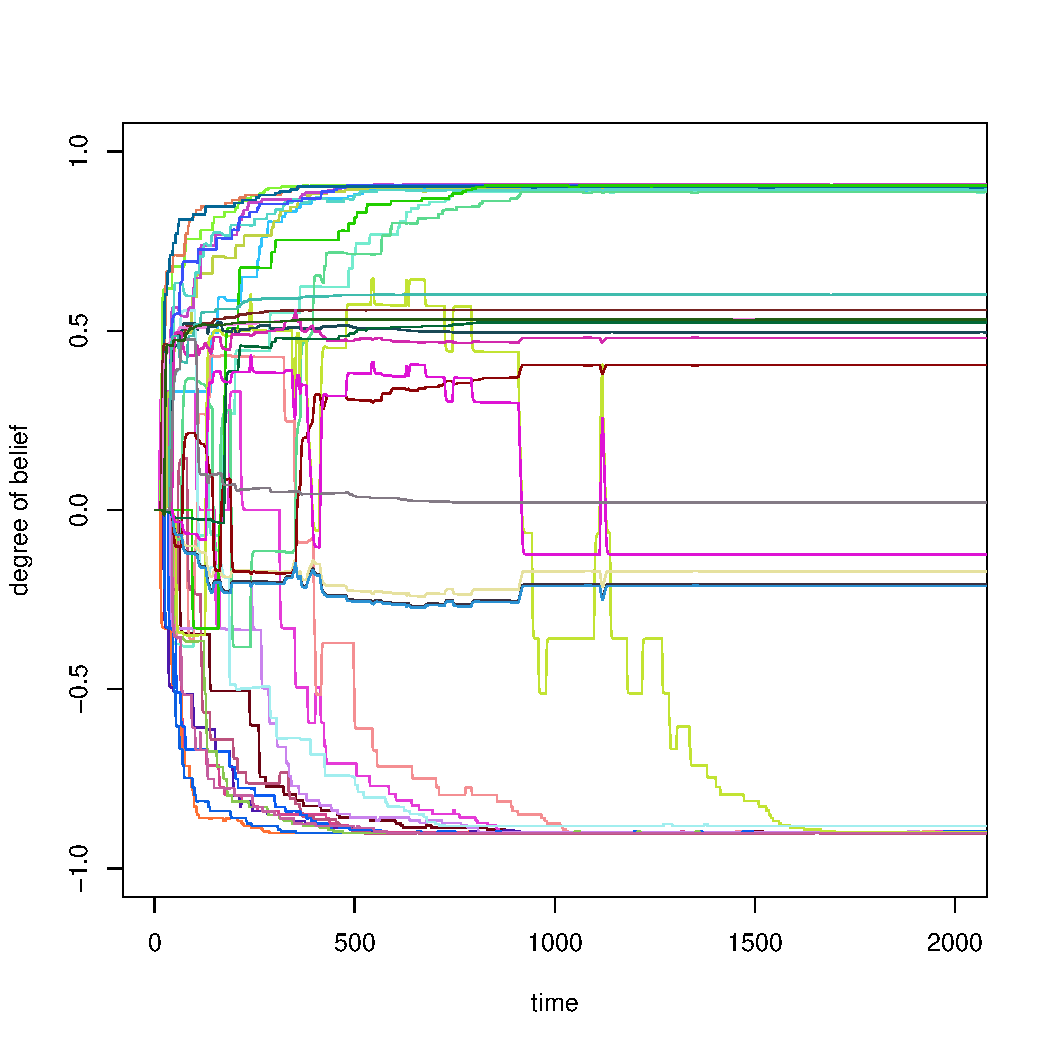
\includegraphics[scale=.20]{../figures/../figures/mra3b2p2000ticksRUN387661242P17} \\
\multicolumn{3}{c}{2000 time steps with same bias\note{ virus bias, earlier sim}} \\
\end{tabular}%
}
\end{frame}

\begin{frame}\frametitle{Transmission biases}
\vspace{-14ex}
\makebox[\textwidth][c]{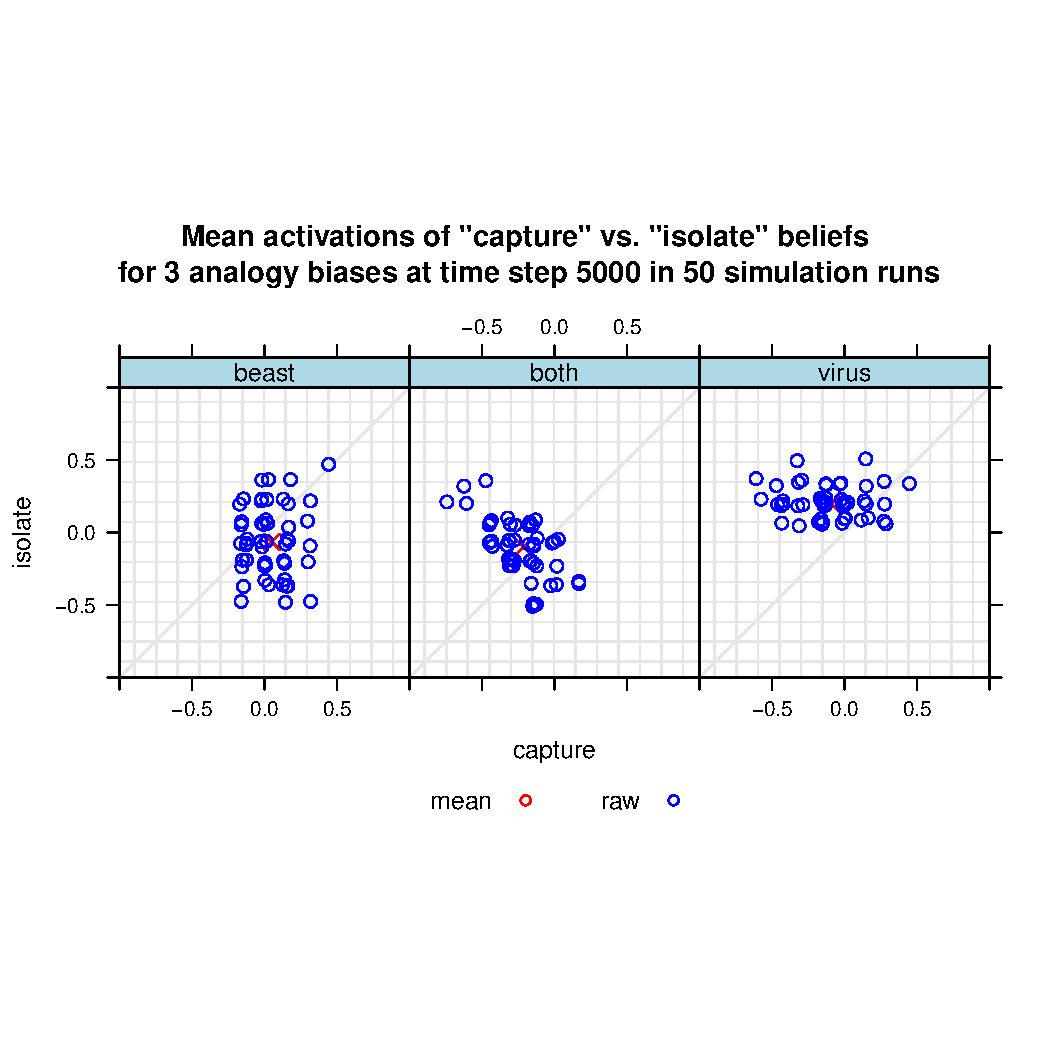
\includegraphics[scale=.7]{../figures/dispersal1threeBiasesWithJitter.pdf}}

\vspace{-16ex}
\begin{center}\tiny (With added noise to show density.)\end{center}
\end{frame}

\begin{frame}{Sanday's correlations}
Using a cross-cultural data set Sanday
\citeyearpar{Sanday:FemalePower} argued for the existence of a
pattern of correlations between several dimensions of cultural
variation:
\ \\
\ \\
\makebox[\textwidth][c]{{\scriptsize
    \begin{tabular}{c|c|c|c}
    \em creator, creation process & \em sex roles (inner/outer) & \em male parenting & \em subsistence importance\\
    \hline\hline male/animal, sky/far, magically & men dominate women & distant, disciplinarian & large game \\
    %\hline couple creates, naturally & intermediate relations & & intermediate/mixed \\
    \hline female, earth/water/body & equal/different & involved, nurturing & gathering/fishing \\
    \hline
    \end{tabular}
}}
\ \\
\ \\
\ \\
Sanday also suggested informal, evocative,
    semi-metaphorical psychological hypotheses about why these
    correlations exist.
\Note{item I've tried to reduce some of these ideas to analogical relationships.}
\end{frame}


\begin{frame}{Sanday's correlations}
How do these correlations between creation stories, male-female
relations, parenting styles, and food gathering methods come
about?
\end{frame}


\begin{frame}\frametitle{Sanday-simulation propositions}
Each person in my POPCO models has:
\begin{itemize}
\item \label{itm:life}Propositions about current human
    interactions:
    \begin{itemize}
    \item \label{itm:parent}Propositions concerning parenting and
        childbirth.
    \item \label{itm:hunt}Propositions concerning large-game
        hunting.
    \end{itemize}
    %
\item \label{itm:origin}Propositions about human origins:
    \begin{itemize}
    \item \label{itm:earth}Propositions characterizing a creator
        who is from the earth, is female, is nurturing, and
        created humans from inside her body.
    \item \label{itm:sky}Propositions characterizing a creator
        who is male, comes from the sky, is both helpful and
        harsh, and created humans magically.
    \end{itemize}
    %
\end{itemize}
\Note{The 37 propositional inputs I use to represent these four domains
(appendix \ref{sec:theinput}) constitute an attempt to provide a
simple and somewhat abstract representation of some of the core
ideas in Sanday's hypotheses. Within each person, POPCO has the
opportunity to map any proposition in set \ref{itm:life} to any
proposition in set \ref{itm:origin}. However, as we'll see, POPCO
agents will  able to construct two distinct sets of analogical
relationships: those relating hunting to sky origin, and those
relating parenting to earth origin.}
\end{frame}


\begin{frame}\frametitle{Analogy as a source of correlations}
\begin{figure}
\centering
    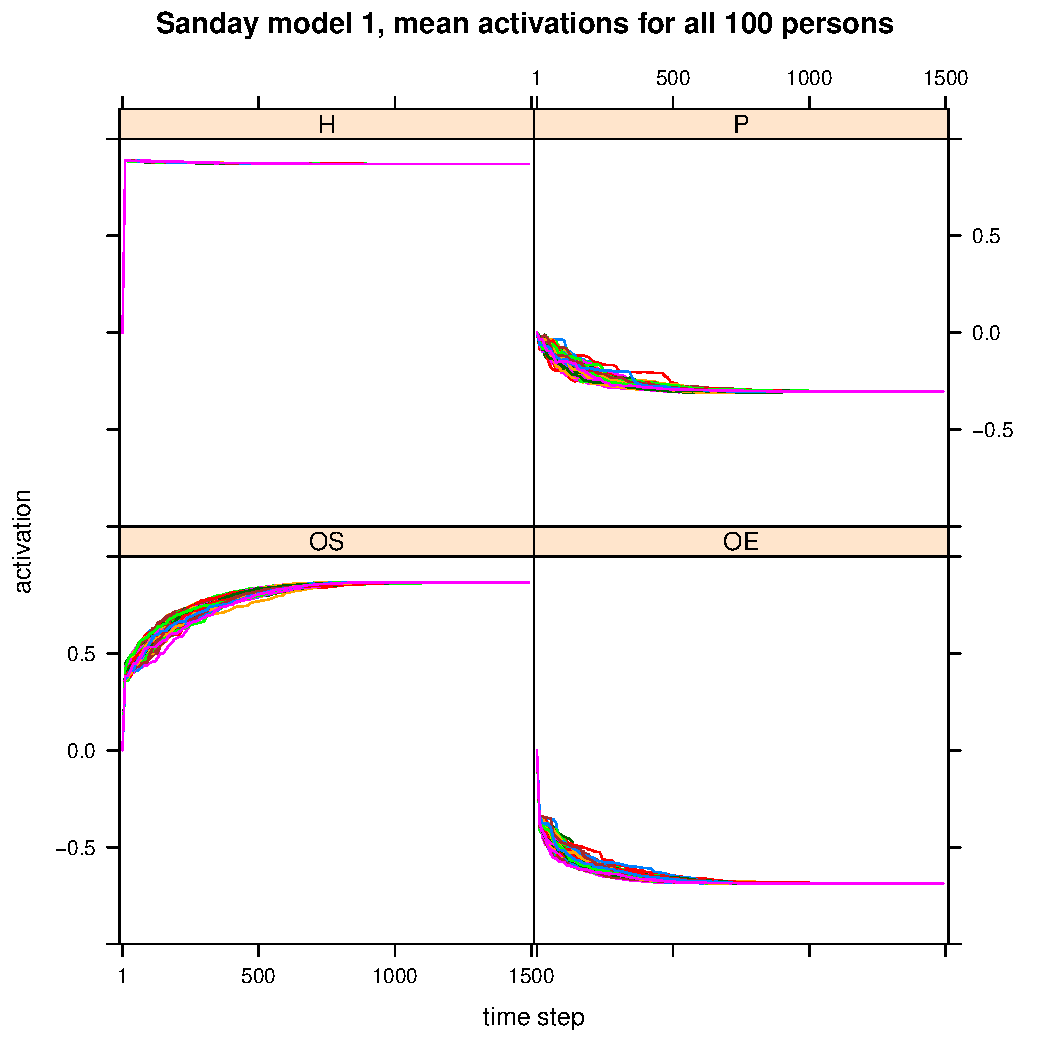
\includegraphics[scale=.45]{../figures/huntingsocDomMeans1500ticksRun11RUN186351490.pdf}
\end{figure} 
\Note{Model 1: Averages of {\em each person's belief
activations in the labeled domain\/}, with hunting propositions
salient during the run.
H: hunting propositions, P: parenting propositions, OS: sky
origin propositions, OE: earth origin propositions.  
One proposition (\lstinline{o-Human-Alive}), common to both OS and OE, is not 
included since it doesn't belong exclusively to either domain.}
\end{frame}


\section{POPCO details}

\begin{frame}\frametitle{POPCO}
\vspace{-3ex}\makebox[\textwidth][c]{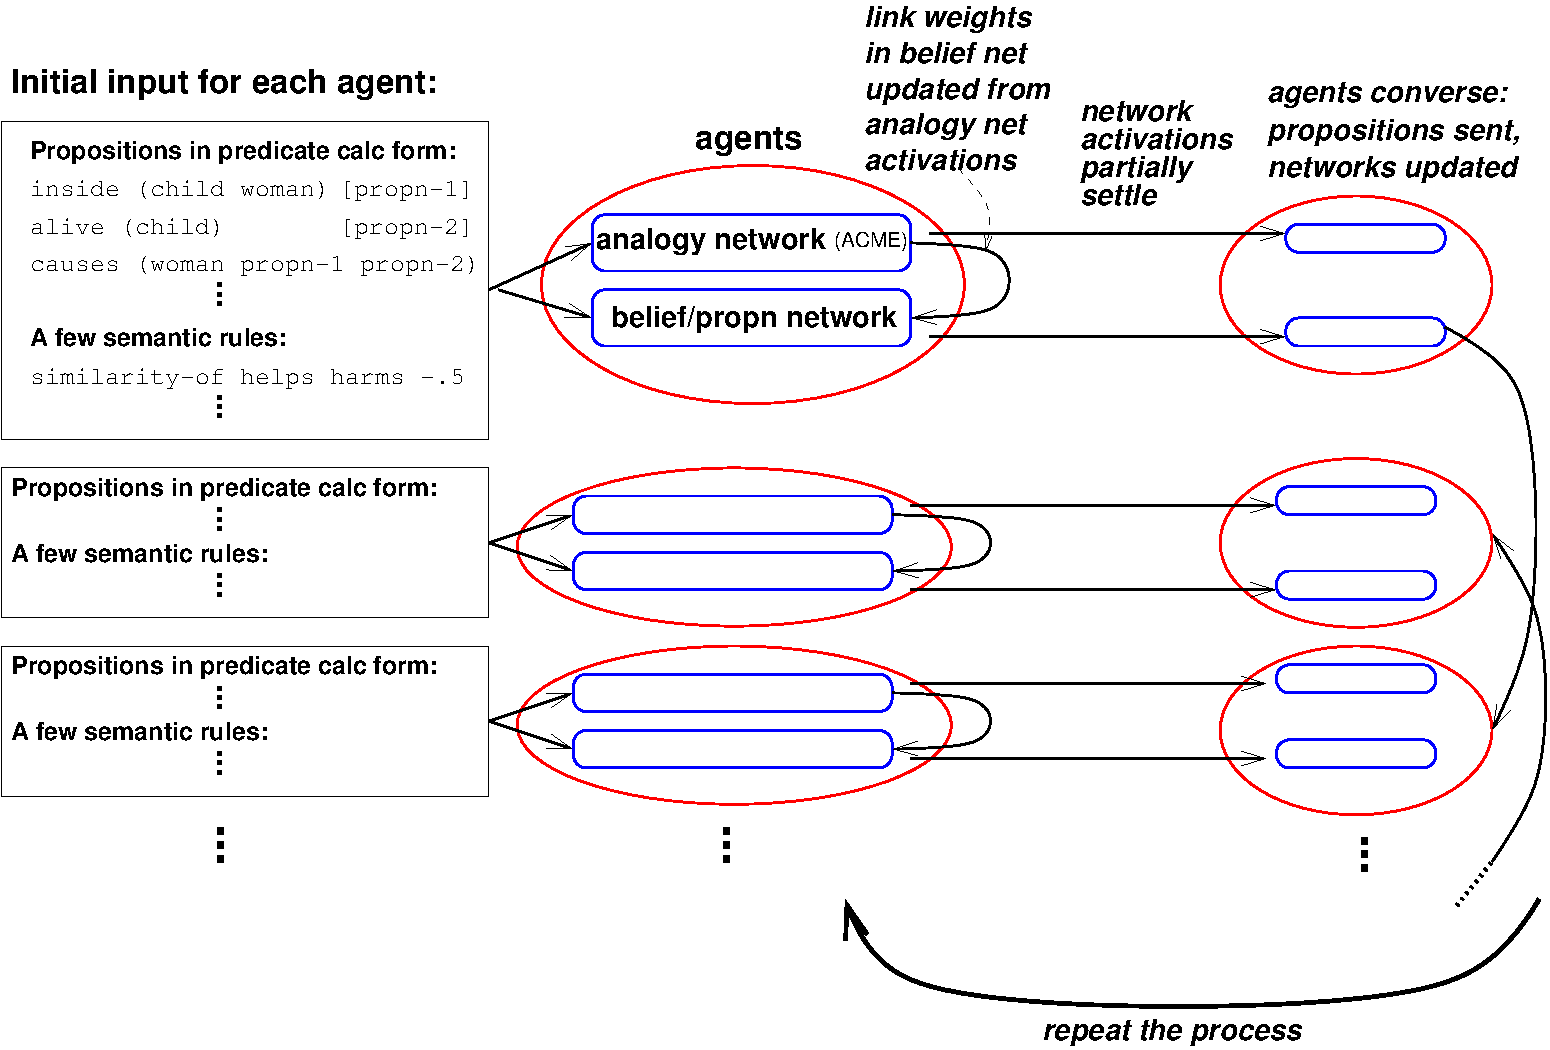
\includegraphics[scale=.40]{../figures/PopcoInternalArchitecture}}\\

\vspace{1ex}
\begin{spacing}{0} % uses setspace package
\scriptsize (Abrams 2013 in {\em Complex Adaptive Systems
Modeling\/}) incorporates ACME \citep{HolyoakThagard:AnalogMapConstraintSat}.\\
\tiny \cf \citep{Gentner:StruMappingThFramework, Hofstadter:FluidConcepts,
WilsonEtAl:STAR2Hiearchically, KokinovPetrov:AMBRmodel}
\end{spacing}
\Note{Original POPCO in Common Lisp.  New POPCO in Clojure,
another dialect of Lisp.  Some people see lisp as foreign and forbidding,
but with a small shift in thinking, lisp is easy, but very
flexible and powerful.  Makes it easy to write programs quickly,
and test and investigate your code and data.  And fun.}
\Note{Each agent has two networks:
Analogy network automatically finds analogies given inputs with
ACME \citep{HolyoakThagard:AnalogMapConstraintSat}; \cf
Gentner/Forbus/Falkenheiner, others.
In proposition network, propositions matched by analogy are more likely to be
believed/disbelieved together.
These networks evolve over time in response to internal processes
and communication.
(Note structures of relations are (almost) all there is to
``meaning".)}
\end{frame}


\begin{frame}\frametitle{Analogy processing}
Possible mappings involved in treating Saddam Hussein in the first
Gulf War (1991) as analogous to Hitler in World War II.
\begin{center}
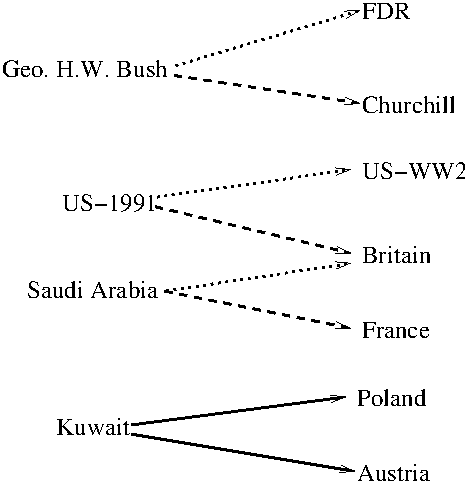
\includegraphics[scale=.65]{../figures/HolyoakThagardMentalLeapsFig5_1.pdf}
\end{center}
{\small After \citep[fig.\ 5.1, p.\ 105]{HolyoakThagard:MentalLeaps}}
\end{frame}

\begin{frame}[fragile]\frametitle{Part of the Iraq analogy}
{\scriptsize
Partial input to network-generation routines in ACME 
\citep{HolyoakThagard:AnalogMapConstraintSat} looks something
like this:\vspace{-2ex}
\begin{verbatim}
president-of (Saddam Iraq)        invade (Iraq Kuwait)
fuhrer-of (Adolph Germany)        occupy (Germany Austria)
\end{verbatim}
}\vspace{1ex}
{\scriptsize Generation of nodes:}
\renewcommand{\arraystretch}{1.65}
\makebox[\textwidth][c]{{\scriptsize
\begin{tabular}{lccccc|}
& \multicolumn{2}{c}{president-of (Saddam Iraq)} && \multicolumn{2}{c}{invade (Iraq Kuwait)} \vspace{1ex} \\
\cline{2-3}\cline{5-6}
\multirow{2}{*}{fuhrer-of (Adolph Germany)\hspace{-1.5ex}} & \multicolumn{2}{|c|}{fuhrer-of \arw president-of}            &&  \multicolumn{2}{|c|}{fuhrer-of \arw invade}\\
                                            & \multicolumn{1}{|c}{\hspace{-2ex}Adolph \arw Saddam\hspace{-2ex}} &  \multicolumn{1}{c|}{\hspace{-3ex}Germany \arw Iraq\hspace{-4ex}} && \multicolumn{1}{|c}{\hspace{-2ex}Adolph \arw Iraq\hspace{-2ex}} & \multicolumn{1}{c|}{\hspace{-3ex}Germany \arw Kuwait\hspace{-4ex}} \\
\cline{2-3}\cline{5-6}\\
\cline{2-3}\cline{5-6}
\multirow{2}{*}{occupy (Germany Austria)\hspace{-3ex}}   & \multicolumn{2}{|c|}{occupy \arw president-of}               && \multicolumn{2}{|c|}{occupy \arw Kuwait} \\
                                            & \multicolumn{1}{|c}{\hspace{-1.5ex}Germany \arw Saddam\hspace{-2ex}} & \multicolumn{1}{c|}{\hspace{-3ex}Austria \arw Iraq\hspace{-4ex}} && \multicolumn{1}{|c}{\hspace{-1.5ex}Germany \arw Iraq\hspace{-2ex}} & \multicolumn{1}{c|}{\hspace{-3ex}Austria \arw Kuwait\hspace{-4ex}} \\
\cline{2-3}\cline{5-6}
\end{tabular}
}}
\end{frame}


\begin{frame}\frametitle{Part of an analogy network}
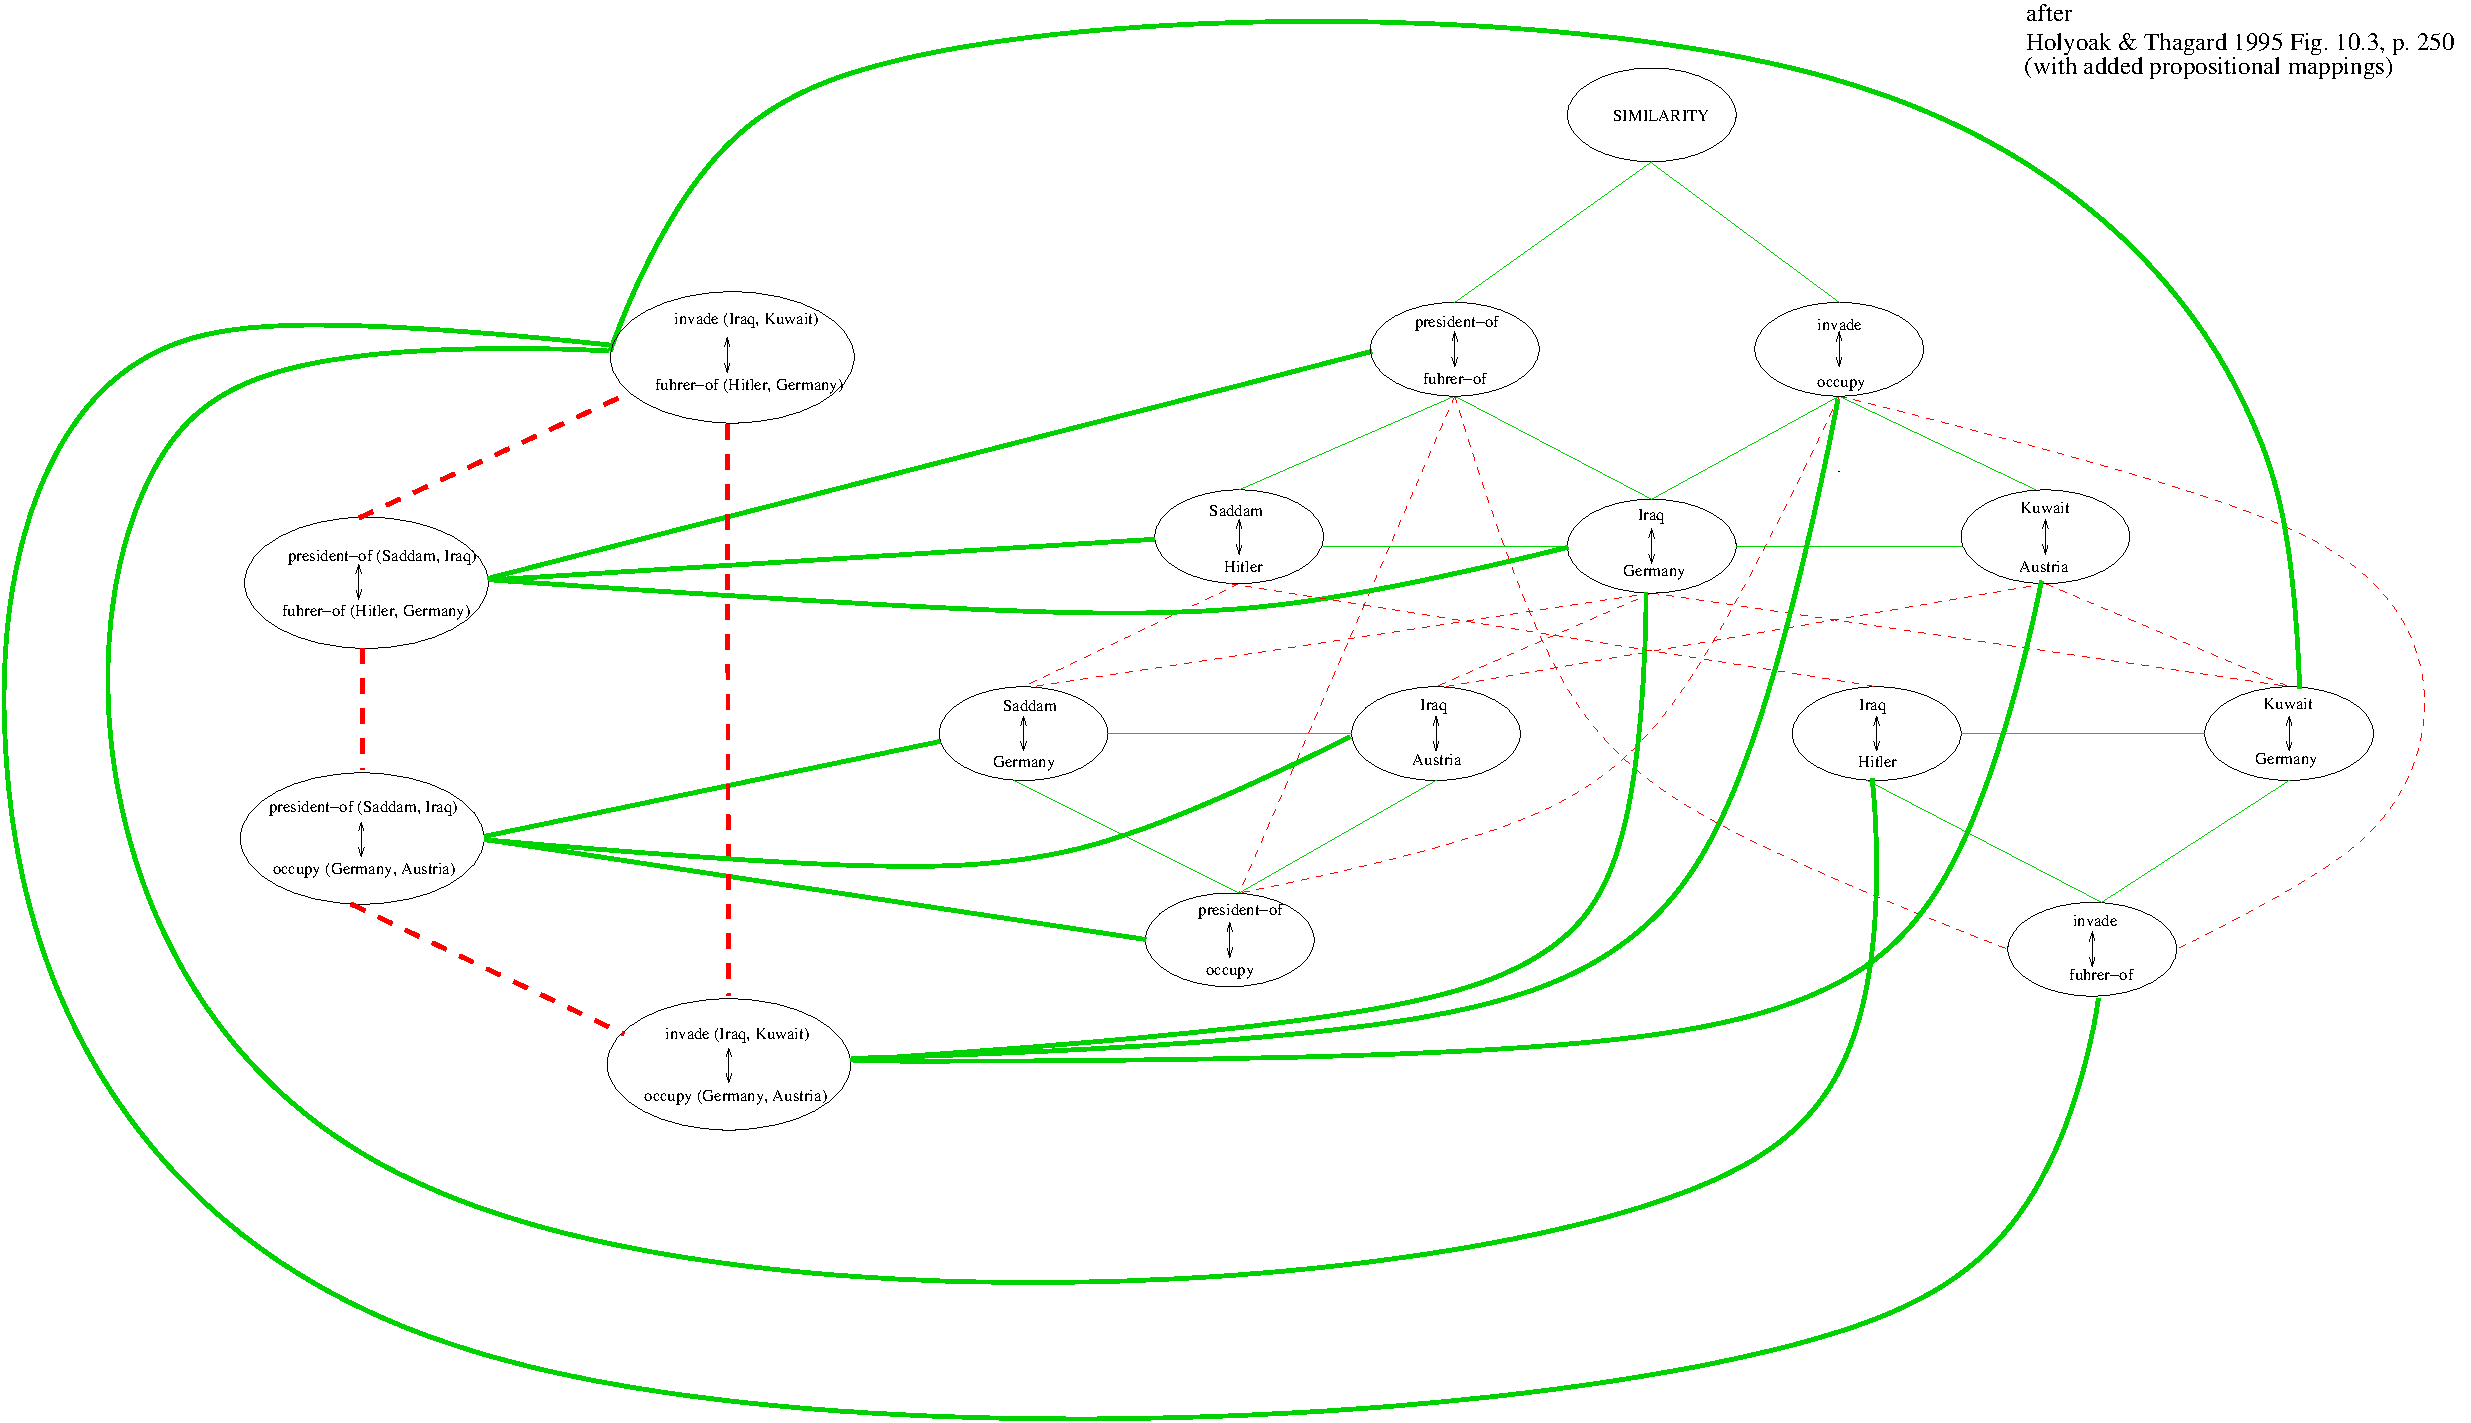
\includegraphics[angle=0,scale=.25]{../figures/HolyoakThagardSimpleIraqNoPurpose.pdf}
\end{frame}


\begin{frame}\frametitle{popco in action}
\begin{center}(MOV files)\end{center}
\end{frame}


\begin{frame}\frametitle{Developing POPCO analogies}
\begin{center}(text files\\
text/crimepropns.nt1\\
text/crime3withnotes.lisp [or sanday])\end{center}
\end{frame}

\lstset{language=Lisp,
  showstringspaces=false,
  basicstyle=\tiny\ttfamily,
  keywordstyle=\bfseries\color{green!40!black},
  commentstyle=\itshape\color{purple!40!black},
  identifierstyle=\color{blue},
  stringstyle=\color{orange},
}

\begin{frame}[fragile]\frametitle{virus, prevention/isolation propositions}
\vspace{-1.5ex}
\begin{lstlisting}
(defvar virus-propns
  '(
    (is-infected (vpers0) v-ip)            ; Person 0 has infection.
    (not-infected (vpers1) v-na)           ; Person 1 lacks infection.
    (is-infected (vpers1) v-ia)            ; Person 1 has infection.
    (harms (vpers1) v-ha)                  ; Person 1 is harmed.
    (cause (v-ia v-ha) v-ci->ha)           ; That person 1 has infection is harmful to person 1. [HO1]
    (infect (vpers0 vpers1) v-ipa)         ; Person 0, who already has infection, infects person 1.
    (cause (v-ipa v-ia) v-ipa->ia)         ; The infecting of person 1 by person 0 causes person 1 to have infection. [HO1]
    (inoculate (vpers1) v-ica)             ; Person 1 gets preventative methods applied, etc., is isolated, etc.
    (prevent (v-ica v-ipa) v-ia->-spa)     ; That person 1 has preventative methods applied prevents person 0 from infecting person 1. [HO1]
    (cause (v-ia->-spa v-na) v-iaspa->na)  ; That the preventative appliction to 1 prevents the infecting, causes [preserves] person 1 lacking infection. [HO2]
    (quarantine (vpers0) v-qp)             ; Person 0 is quarantined.
    (prevent (v-qp v-ipa) v-qp->-spa)      ; That person 0 is quarantined prevents person 0 from infecting person 1.
    (cause (v-qp->-spa  v-na) v-qpspa->na) ; That (quarantining 0 prevents 0 from infecting 1) causes [preserves] person 1 lacking infection. [HO2]
   ))

(defvar viral-crime-propns
  '(
    (is-criminal (cpers0) cv-cp)              ; Garden 0 has been attacked by pests.
    (not-criminal (cpers1) cv-na)             ; Garden 1 has not been attacked by pests.
    (is-criminal (cpers1) cv-ca)              ; Garden 1 has been attacked by pests.
    (harms (cpers1) cv-ha)                    ; Garden 1 is harmed.
    (cause (cv-ca cv-ha) cv-ca->hp)           ; Garden 1 being attacked by pests is harmful to garden 1.
    (recruit (cpers0 cpers1) cv-rpa)          ; Pests move from garden 0 to garden 1.
    (cause (cv-rpa cv-ca) cv-sca->ca)         ; Pests moving from garden 0 to garden 1 causes garden 1 to be attacked. [HO1]
    (support (cpers1) cv-sa)                  ; Garden 1 is protected by fertilizer, substances noxious to pests, fences, etc.
    (prevent (cv-sa cv-rpa) cv-sa->-rpa)      ; Garden 1 being protected prevents pests from moving from garden 0 to garden 1. [HO1]
    (cause (cv-sa->-rpa cv-na) cv-sarpa->na)  ; That garden 1 is protected pests from moving from 0 to 1 causes [preserves] 1's health. [HO2]
    (imprison (cpers0) cv-ip)                 ; Garden 0 is isolated by fences, etc.
    (prevent (cv-ip cv-rpa) cv-ip->-rpa)      ; Garden 0 being isolated prevents pests from moving from garden 0 to garden 1. [HO1]
    (cause (cv-ip->-rpa  cv-na) cv-iprpa->na) ; That O's isolation prevents pests from moving from 0 to 1 causes [preserves] 1's health. [HO2]
   ))

\end{lstlisting}
\end{frame}

\begin{frame}[fragile]\frametitle{beast, capture propositions}
\begin{lstlisting}
(defvar beast-propns
  '(
    (human (bpers) b-pp)                  ; Person is human. [should match cb-np]
    (aggressive (beast) b-ab)             ; Beast is agressive.
    (attack (beast bpers) b-abp)          ; Beast attacks person.
    (cause (b-ab b-abp) b-ab->abp)        ; Beast's agressiveness causes it to attack person. [HO1]
    (harms (bpers) b-hp)                  ; Person is harmed.
    (cause (b-abp b-hp) b-abp->hp)        ; Beast attacking human harms person. [HO1]
    (helps (beast) b-hb)                  ; Beast is benefited.
    (cause (b-abp b-hb) b-abp->hb)        ; Beast attacking person benefits beast. [HO1]
    (capture (bpers beast) b-cpb)         ; Person captures beast.
    (prevent (b-cpb b-abp) b-cpb->-abp)   ; Person capturing beast prevents beast attacking person. [HO1]
    (danger-to (bpers) b-dtp)             ; Person is subject to danger.
    (cause (b-cpb b-dtp) b-cpb->dtp)      ; Person capturing beast is dangerous to person. [HO1]
   ))

(defvar beastly-crime-propns
  '(
    (not-criminal (cpers) cb-np)
    (aggressive (crim-pers) cb-ap)
    (victimize (crim-pers cpers) cb-vpp)
    (cause (cb-ap cb-vpp) cb-ap->vpp)
    (harms (cpers) cb-hcp)
    (cause (cb-vpp cb-hcp) cb-vpp->hcp)
    (helps (crim-pers) cb-hp)
    (cause (cb-vpp cb-hp) cb-vpp->hp)
    (capture (cpers crim-pers) cb-cpc)
    (prevent (cb-cpc cb-vpp) cb-cpc->-vpp)
    (danger-to (cpers) cb-dtp)
    (cause (cb-cpc cb-dtp) cb-cpc->dtp)
   ))
\end{lstlisting}
\end{frame}

\begin{frame}[fragile]\frametitle{Additional semantic specifications}
\begin{lstlisting}
(defvar semantic-relations
  '(
    (similar 'cause 'prevent (* -1 *ident-weight*)) ; avoid mapping cause to prevent
    (similar 'is-beastly 'is-infected (* -1 *ident-weight*))
    (semantic-iff 'cb-vpp 'v-ipa -.1) ; kludge, prevent mapping
    (semantic-iff 'cv-rpa 'b-abp -.1) ; keeps code simpler
   ))
\end{lstlisting}
\end{frame}



\begin{frame}\frametitle{Internal effects of analogies}
\vspace{-6ex}\tiny\sf
\makebox[\textwidth][c]{%
\begin{tabular}{rl}
\vspace{6ex}
\multirow{24}{*}{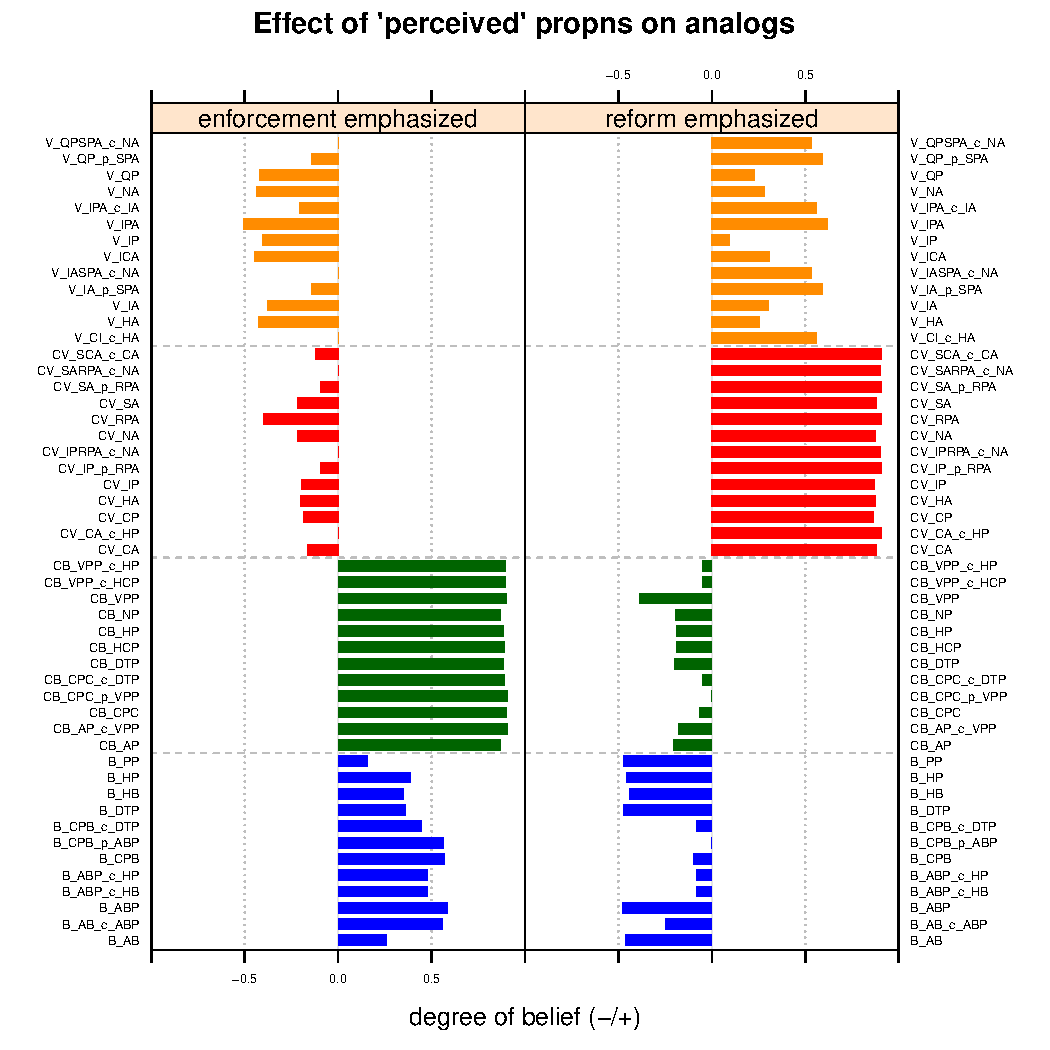
\includegraphics[scale=.45]{../figures/crime3basicCheckCrimePerceiversOnly}} & \\
& \\
& \\
& \\
& \\
& \hspace{-4ex}virus \\
& \\
& \\
& \\
& \\
& \\
& \hspace{-4ex}crime reform \\
& \\
& \\
& \\
& \\
& \\
& \hspace{-4ex}crime enforcement \\ 
& \\
& \\
& \\
& \\
& \\
& \hspace{-4ex}beast \\
\end{tabular}%
}
\end{frame}


\begin{frame}\frametitle{}
\scalebox{0.75}{%
{\tiny
\begin{tabular}{llll}
\sc Predicate &\hspace{-3ex} \sc Arguments &\hspace{-3ex} \sc Proposition name &\hspace{-3ex} \sc Intended meaning\\
\hline\hline
\em Parenting : \\
\hline 1. alive &\hspace{-3ex} (child) &\hspace{-3ex}  \em p-Child-Alive &\hspace{-3ex} A child is alive. \\
\hline 2. intimate-agent &\hspace{-3ex} (woman, child) &\hspace{-3ex}  \em p-Child-Close &\hspace{-3ex} Women, children are emotionally intimate. \\
\hline 3. inside &\hspace{-3ex} (child, woman) &\hspace{-3ex}  \em p-Protochild-Inside &\hspace{-3ex} A child (fetus) is initially inside a woman. \\
\hline 4. process-from-to &\hspace{-3ex} ({\em p-Protochild-Inside, p-Child-Alive}) &\hspace{-3ex}  \em p-Child-From-Within-Woman &\hspace{-3ex} There is a process that leads from (3) to (1). \\
\hline 5. creates &\hspace{-3ex} (woman, {\em p-Child-From-Within-Woman}) &\hspace{-3ex}  \em p-Woman-Creates-Child-From-Within &\hspace{-3ex} Woman are the cause of the process in (4). \\
\hline 6. natural-process &\hspace{-3ex} ({\em p-Woman-Creates-Child-From-Within}) &\hspace{-3ex}  \em p-Woman-Creates-Naturally &\hspace{-3ex} The preceding process is natural. \\
\hline 7. helps &\hspace{-3ex} (woman, child) &\hspace{-3ex}  \em p-Woman-Helps-Child &\hspace{-3ex} Women help (nurture, etc.) their children. \\
\hline 8. causes &\hspace{-3ex} (nothing, {\em p-Woman-Helps-Child}) &\hspace{-3ex}  \em p-Woman-Nurtures &\hspace{-3ex} Nothing causes women to nurture children. \\
\hline 9. nothing &\hspace{-3ex} (nothing) &\hspace{-3ex}  \em p-Nothing  &\hspace{-3ex} (Has no real meaning, but is useful.) \\
\hline\hline \em Hunting: \\
\hline 10. feels-power &\hspace{-3ex} (man) &\hspace{-3ex}  \em h-Man-Power &\hspace{-3ex} Men feel powerful, able to control nature. \\
\hline 11. power-source &\hspace{-3ex} (game, {\em h-Man-Power}) &\hspace{-3ex}  \em h-Game-Power-Source &\hspace{-3ex} Game is a source of this power. \\
\hline 12. mysterious-process &\hspace{-3ex} ({\em h-Game-Power-Source}) &\hspace{-3ex}  \em h-Game-Power-Mysteriously &\hspace{-3ex} Game being source of power is mysterious. \\
\hline 13. hunts-endangers &\hspace{-3ex} (man, game) &\hspace{-3ex}  \em h-Man-Endangers-Game &\hspace{-3ex} Men hunting is dangerous to game. \\
\hline 14. harms &\hspace{-3ex} (game, man) &\hspace{-3ex}  \em h-Game-Harms-Man &\hspace{-3ex} Game sometimes harms men. \\
\hline 15. causes &\hspace{-3ex} ({\em h-Man-Endangers-Game, h-Game-Harms-Man}) &\hspace{-3ex}  \em h-Hunting-Is-Dangerous &\hspace{-3ex} (13) is a cause of (14) \\
\hline 16. hunts-skillfully &\hspace{-3ex} (man, game) &\hspace{-3ex}  \em h-Skillful-Hunting &\hspace{-3ex} Hunting involves skill. \\
\hline 17. helps &\hspace{-3ex} (game, man) &\hspace{-3ex}  \em h-Game-Provides &\hspace{-3ex} Game helps men (by providing food, etc.). \\
\hline 18. causes &\hspace{-3ex} ({\em h-Skillful-Hunting, h-Game-Provides}) &\hspace{-3ex}  \em h-Hunting-Rewards-Skill &\hspace{-3ex} Skill in hunting causes game's benefit.\\
\hline 19. distant-agent &\hspace{-3ex} (game, man) &\hspace{-3ex}  \em h-Game-Distant &\hspace{-3ex} Game and men are emotionally distant. \\
\hline\hline
\em Both origin domains: \\
\hline 
20. alive &\hspace{-3ex} (human) &\hspace{-3ex}  \em o-Human-Alive &\hspace{-3ex} Humans are alive. \\
\hline\hline
\em Earth origin: \\
\hline 21. inside &\hspace{-3ex} (human, e-god) &\hspace{-3ex}  \em oe-Protohuman-Inside &\hspace{-3ex} Human(s) began inside e-god. \\
\hline 22. process-from-to &\hspace{-3ex} ({\em oe-Protohuman-Inside, o-Human-Alive}) &\hspace{-3ex}  \em oe-Human-From-Within-God &\hspace{-3ex} There's a process leading from (21) to (20). \\
\hline 23. causes &\hspace{-3ex} (e-god, {\em oe-Human-From-Within-God}) &\hspace{-3ex}  \em oe-God-Creates-Human-From-Within &\hspace{-3ex} An e-god causes this process. \\
\hline 24. natural-process &\hspace{-3ex} ({\em oe-God-Creates-Human-From-Within}) &\hspace{-3ex}  \em oe-God-Creates-Naturally &\hspace{-3ex} An e-god doing so is a natural process. \\
\hline 25. helps &\hspace{-3ex} (e-god, human) &\hspace{-3ex}  \em oe-God-Helps-Human &\hspace{-3ex} An e-god helps humans, is nurturing, etc. \\
\hline 26. causes &\hspace{-3ex} (nothing, {\em oe-God-Helps-Human}) &\hspace{-3ex}  \em oe-God-Nurtures &\hspace{-3ex} Nothing causes an e-god to be nurturing. \\
\hline 27. close &\hspace{-3ex} (e-god, human) &\hspace{-3ex}  \em oe-Earthly-God &\hspace{-3ex} e-god is physically close to humans. \\
\hline 28. nothing &\hspace{-3ex} (nothing) [Has no real meaning, but is useful.]&\hspace{-3ex}  \em oe-Nothing &\hspace{-3ex}  (Has no real meaning, but is useful.) \\
\hline\hline
\em Sky origin: \\
\hline 29. creates &\hspace{-3ex} (s-god, {\em o-Human-Alive}) &\hspace{-3ex}  \em os-God-Creates-Human &\hspace{-3ex} An s-god causes (20). \\
\hline 30. mysterious-process &\hspace{-3ex} ({\em os-God-Creates-Human}) &\hspace{-3ex}  \em os-God-Creates-Mysteriously &\hspace{-3ex} The process in (29) is a mysterious process. \\
\hline 31. offends &\hspace{-3ex} (human, s-god) &\hspace{-3ex}  \em os-Human-Offends-God &\hspace{-3ex} Humans offend s-god (sometimes). \\
\hline 32. harms &\hspace{-3ex} (s-god, human) &\hspace{-3ex}  \em os-God-Harms-Human &\hspace{-3ex} s-god harms humans (sometimes). \\
\hline 33. causes &\hspace{-3ex} ({\em os-Human-Offends-God,\, os-God-Harms-Human}) &\hspace{-3ex}  \em os-Offense-Causes-Punishment &\hspace{-3ex} Offending s-god causes punishment. \\
\hline 34. supplicates &\hspace{-3ex} (human, s-god) &\hspace{-3ex}  \em os-Human-Supplicates &\hspace{-3ex} Humans supplicate, pray, etc.\ to s-god. \\
\hline 35. helps &\hspace{-3ex} (s-god, human) &\hspace{-3ex}  \em os-God-Helps-Human &\hspace{-3ex} s-god helps humans (sometimes). \\
\hline 36. causes &\hspace{-3ex} ({\em os-Human-Supplicates, os-God-Helps-Human}) &\hspace{-3ex}  \em os-God-Rewards &\hspace{-3ex} Supplicating is what causes s-god to help. \\
\hline 37. distant &\hspace{-3ex} (s-god, human) &\hspace{-3ex}  \em os-Heavenly-God &\hspace{-3ex} s-god is physically distant from humans. \\
\hline\hline
\end{tabular}}}
\end{frame}


\begin{frame}\frametitle{Sanday-sim semantic specs}
{\scriptsize
(similar 'helps 'harms (* -1 *ident-weight*))\\
(similar 'feels-power 'alive (* -.75 *ident-weight*))\\
(similar 'woman 'human (* .5 *ident-weight*))\\
(similar 'man 'human (* .5 *ident-weight*))\\
(similar 'distant 'distant-agent (* .5 *ident-weight*))\\
(similar 'close 'intimate-agent (* .5 *ident-weight*))\\
(similar 'offends 'harms (* .5 *ident-weight*))\\
(semantic-iff 'oe-Earthly-God 'os-Heavenly-God -.5)\\
(semantic-iff 'oe-God-Creates-Naturally 'os-God-Creates-Mysteriously -.5)\\
(semantic-iff 'os-Heavenly-God 'os-God-Creates-Mysteriously .1)\\
(semantic-iff 'oe-God-Creates-Naturally 'oe-God-Creates-Human-From-Within .5)\\
(semantic-iff 'oe-God-Nurtures 'oe-God-Creates-Human-From-Within .1)\\
(semantic-iff 'oe-Human-From-Within-God 'oe-God-Creates-Human-From-Within .5)\\
(semantic-iff 'oe-God-Creates-Human-From-Within 'os-God-Creates-Human-From-Object -.5)
}
\end{frame}


\begin{frame}\frametitle{How to get started}
\begin{itemize}
\item NetLogo is free, includes many example programs to use
as starting points.
\item NetLogo site has tutorials.
\item I recommend R (graphics, statistics), Gephi
(network graphics and analysis).
\end{itemize}
\end{frame}

\begin{frame}\frametitle{How to get started}
\begin{itemize}
\item For more flexibility, Clojure and other lisps are high-level, flexible
languages that allow poking around in your data and
investigating newly-changed code on the fly
\item Clojure makes it easy to use Java libraries (software
tools), and can generate Javascript code.
\item There are good books and tutorials.
\end{itemize}
\end{frame}

\begin{frame}\frametitle{How to get started}
\begin{itemize}
\item I mentioned various simulations used in literature studies,
history, and philosophy.  I'm happy to provide references.
\item Please talk to me about POPCO if interested.\\
\item My ``A Moderate Role for Cognitive Models in Agent-Based Modeling of
Cultural Change" in {\em Complex Adaptive Systems Modeling\/} 
\citeyear{Abrams:ModerateRole} has details on POPCO and references
on analogy, etc.
\end{itemize}
\end{frame}


\begin{frame}\frametitle{Current project}
Current POPCO project is on interactions between sustainable farming practices and religious traditions in Bali.
\end{frame}

\begin{frame}%
  \titlepage%
\end{frame}

\begin{frame}[allowframebreaks]\frametitle{References}
\def\newblock{}  % beamer kludge
\bibliographystyle{myforthcoming} % the .bst file
\bibliography{phil}
\end{frame}

\end{document}


